\documentclass[10pt, twocolumn]{article}
\usepackage{nameref}
\usepackage[dvipsnames]{xcolor}
\usepackage{graphicx} 
\graphicspath{{Figures/}}
\usepackage[left=1in,right=1in,top=1in]{geometry}
\usepackage[breaklinks]{hyperref}
\usepackage{microtype}
\usepackage{tikz}
\usepackage{natbib}
\usepackage{multicol}
\usepackage{amsmath}
\usepackage{JML}
\usepackage{amssymb}
\usetikzlibrary{decorations.pathreplacing,calligraphy}

\title{Jack's Machine Learning Notes}
\author{Jack Fraser-Govil}
\renewcommand\vec[1]{\boldsymbol{\textbf{#1}}}
\newcommand\cec[1]{\tilde{\vec{#1}}}
\begin{document}
	\maketitle{}

	\section{Perceptrons}

		The first `Machine Learning' tool was the \textit{perceptron}, which is a form of a binary classifier: given a vector (representing `features' of a dataset), it could assign either a 0 or a 1 to it, indicating membership of one group or another. 

		The perceptron algorithm is highly simple:
		\begin{equation}
			\mathcal{P}_{b,\vec{w}}(\vec{x}) = \text{Perceptron}(\vec{x}) = \begin{cases} 1 & \text{if } \vec{w} \cdot \vec{x} + b > 0 \\ 0 & \text{else} \end{cases}
		\end{equation}
		This, in essence, splits the $d$-dimensional domain into two by defining a hyperplane ($d-1$ dimensional): those which lie one one side of the hyperplane fall into one category, those which lie on the other side are not in that category. 
		
		\subsection{Biases \& Dimensionality}
		Note that, strictly speaking, we do not need the `bias' term, $b$ -- the vector $\vec{w}$ is sufficent to define the hyperplane. In fact, as a general statement you only require $d$ parameters to split the $d$-dimensional plane into two. 
		
		Indeed, we see that including $b$ makes the solution degenerate, since $(\alpha \vec{w}) \cdot \vec{x} + \alpha b$ gives identical classifications for all $\alpha > 0$ since our classifications are based only on when this value is greater than 0. We could therefore divide all of our solutions by $b$ and simply look for when the perceptron value was greater than or less than 1. So why is the `bias' term $b$ included?
		
		The answer is twofold. Firstly, keeping the $b$ separate makes the convergence of the algorithm quicker since it (by comparison with the 2D case $y= mx + b$) allows us to move the hyperplane `vertically' in space, without altering the gradient of the plane: if only $\vec{w}$ was used, simple translations would require simultaneous alterations of all values in the vector. 
		
		Secondly, it also prevents the numerical issues which are encountered when (using the 2D case as an example), $m\to\infty$ for a vertical line -- using $\vec{w}$ and $b$ instead of just $m$ and $c$ does not require the infinity. Thus allowing for degenerate solutions has its advantages. 
		
		\subsection{Training}

		`Training' the perceptron amounts to finding the value of $\vec{w}$ and $b$ (for simplicity, we will refer to this combination as $\cec{w} = [b,\vec{w}]$, where $\cec{x} = [1,\vec{x}]$) which produces the smallest number of errors. 

		For each datum $j$ in the training dataset, where $\vec{x}_j$ is the features and $d_j$ is the (correct) label, the weights are updated as follows:
		\begin{equation}
			\cec{w} \to \cec{w} + r \left( d_j - \mathcal{P}_{\cec{w}}(\vec{x}_j) \right) \cec{x}
		\end{equation}
		Where $r$ is the `learning rate'. In short: whenever the Perceptron makes a mistake ($d_j \neq \mathcal{P}$), it updates its vectors slightly in the direction which makes it less-incorrect.

		When an optimal solution exists (see later), this algorithm is guaranteed to converge to the global optimum, though the choice of the learning rate $r$ can affect how rapidly that convergence occurs.

		\subsection{Extensions \& Limitations}

			In the simple case of a 2D classifier, the naive perceptron is limited to simply drawing straight lines (`decision boundaries') through the data - a clear limitation of the method which extends to arbitrarily high dimensions. You can, however, get a bit cleverer.
			
			Imagine that, in our 2D case, you have some which looks like it has a quadratic decision boundary. Rather than feeding in $(x,y)$, you feed in $(x,x^2,y)$ into a new 3D perceptron, such that you are comparing $w_0 y + w_1 x + w_2 x^2 + b >? 0$. This model \textbf{is} capable of learning the quadratic decision boundary -- however, you had to feed in the non-linearity manually. This can extend to arbitrarily complex models -- even if the data is only 2D in reality, you could feed in the vector $\vec{x} = (x,y,\sin(x), \cos^2(x), xy, x^9.04 e^y \hdots)$, which would allow the model to tune to arbitrary decision boundaries -- those familiar with basis functions might suggest that something along the lines of $(y,x,x^2-1,x^3-3x,x^406x^2+3)$ (i.e. the Hermite polynomials) would be an appropriate choice, since -- when enough dimensions are included -- they can arbitrarily approximate any function.

			However, the Perceptron has a fundamental flaw, insofar that, no matter how clever you get with transforming your input data, it remains a \textit{linear} classifier: the operation $\cec{w} \cdot \cec{x}$ amounts to splitting your projected space in two: if the data is not ``linearly separable'', then the Perceptron will only be able to make crude approximations.
			
			A simple example of a function which is not linearly separable is the XOR operation: a famous 1969 book (Minsky \& Papert) proved this result definitively, which led to a pause in the development of machine learning for more than 10 years. 

	\section{Feedforward Neural Networks}
	\begin{figure*}[t]
		\begin{center}

		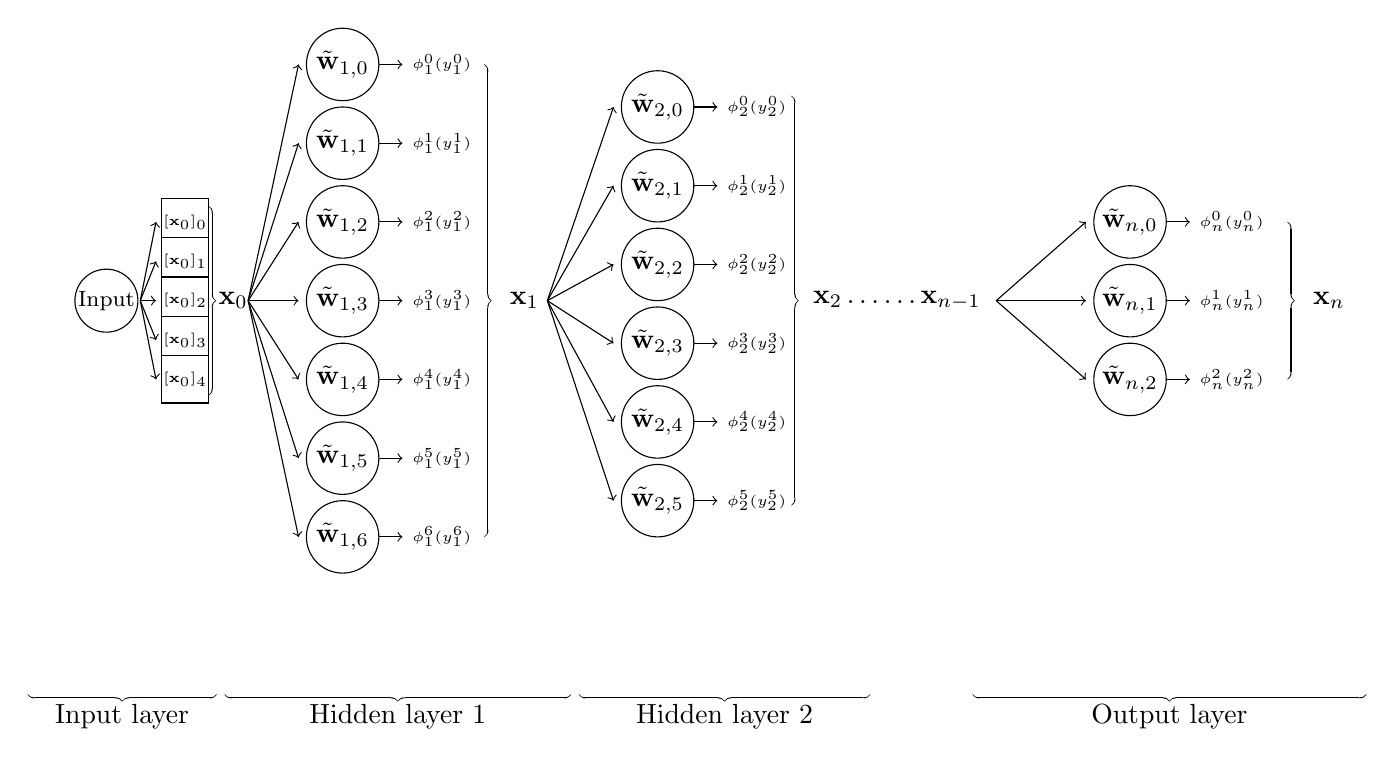
\begin{tikzpicture}
			\draw (0,0) circle (0.4);
			\node at (0,0) {\footnotesize Input};
			\foreach \i[count=\j from 0] in {2,1,...,-2}
			{
				\def\r{0.3}
				\def\y{\i/2}
				\def\x{1}
				\draw[->] (0.43,0)--({\x-\r-0.07},\y);
				\draw[fill=white] ({\x-\r},{\y-\r})--({\x+\r},{\y-\r})--({\x+\r},{\y+\r})--({\x-\r},{\y+\r})--cycle;
				\node at (\x,{\y}) {\fontsize{1}{0}\selectfont $[\vec{x}_0]_\j$};
			}
			\def\baseheight{-5}
			\draw [decorate, decoration = {calligraphic brace}] (1.4,\baseheight) --node[below]{Input layer}  (-1,\baseheight);
			\draw [decorate, decoration = {calligraphic brace}] (5.9,\baseheight) --node[below]{Hidden layer 1}  (1.5,\baseheight);
			\draw [decorate, decoration = {calligraphic brace}] (9.7,\baseheight) --node[below]{Hidden layer 2}  (6,\baseheight);
			\draw [decorate, decoration = {calligraphic brace}] (16,\baseheight) --node[below]{Output layer}  (11,\baseheight);
			\draw [decorate, decoration = {calligraphic brace}] (1.3,1.2) --  (1.3,-1.2);
			\node[anchor=west] at (1.3,0) {$\vec{x}_0$};

			\foreach \i[count=\j from 0] in {3,2,...,-3}
			{
				\def\r{0.46}
				\def\y{\i}
				\def\x{3}
				\draw[->] (1.8,0)--({\x-\r-0.1},\y);
				\draw (\x,{\y}) circle ({\r});
				\node at (\x,{\y}) { $\cec{w}_{1,\j}$};
				\draw [->] ({\x+\r},{\y})--({\x+\r+0.3},{\y});
				\def\xx{\x+\r+0.3}
				% \draw[fill=white] ({\x-\r},{\y-\r})--({\x+\r},{\y-\r})--({\x+\r},{\y+\r})--({\x-\r},{\y+\r})--cycle;
				\node[anchor=west] at (\xx,{\y}) {\fontsize{1}{0}\selectfont$\phi_{1}^{\j}(y_{1}^{\j})$};
			}
			\draw [decorate, decoration = {calligraphic brace}] (4.8,3) --  (4.8,-3);
			
			\node[anchor=west] at (5,0) {$\vec{x}_1$};

			\foreach \i[count=\j from 0] in {2,1,0,-1,-2,-3}
			{
				\def\r{0.46}
				\def\y{\i+\r}
				\def\x{7}
				\draw[->] (5.6,0)--({\x-\r-0.1},\y);
				\draw (\x,{\y}) circle ({\r});
				\node at (\x,{\y}) { $\cec{w}_{2,\j}$};
				\draw [->] ({\x+\r},{\y})--({\x+\r+0.3},{\y});
				\def\xx{\x+\r+0.3}
				% \draw[fill=white] ({\x-\r},{\y-\r})--({\x+\r},{\y-\r})--({\x+\r},{\y+\r})--({\x-\r},{\y+\r})--cycle;
				\node[anchor=west] at (\xx,{\y}) {\fontsize{1}{0}\selectfont$\phi_{2}^{\j}(y_{2}^{\j})$};
			}
			\draw [decorate, decoration = {calligraphic brace}] (8.7,2.6) --  (8.7,-2.6);
			\node[anchor=west] at (8.85,0) {$\vec{x}_2\hdots\hdots\vec{x}_{n-1}$};
			\foreach \i[count=\j from 0] in {1,0,-1}
			{
				\def\r{0.46}
				\def\y{\i}
				\def\x{13}
				\draw[->] (11.3,0)--({\x-\r-0.1},\y);
				\draw (\x,{\y}) circle ({\r});
				\node at (\x,{\y}) { $\cec{w}_{n,\j}$};
				\draw [->] ({\x+\r},{\y})--({\x+\r+0.3},{\y});
				\def\xx{\x+\r+0.3}
				% \draw[fill=white] ({\x-\r},{\y-\r})--({\x+\r},{\y-\r})--({\x+\r},{\y+\r})--({\x-\r},{\y+\r})--cycle;
				\node[anchor=west] at (\xx,{\y}) {\fontsize{1}{0}\selectfont$\phi_{n}^{\j}(y_{n}^{\j})$};
			}
			\draw [decorate, decoration = {calligraphic brace}] (15,1) --  (15,-1);
			\node[anchor=west] at (15.2,0) {$\vec{x}_{n}$};
		\end{tikzpicture}
		
		\end{center}
	\end{figure*}
		The failure of peceptrons was twofold: the was only a single neuron (and hence a single division of the plane), and they were discontinuous (they were either right or wrong, they couldn't move smoothly between these options). The Multi-Layer Perceptron solves this problem by chaining together several modified perceptrons, and has three components:

		\begin{itemize}
			\item \textbf{Input Layer}: performs preprocessing on the input, transforming it into (usually) a 1D feature vector
			\item \textbf{Hidden Layers}: several layers of perceptron `neurons'
			\item \textbf{Output Layers}: The final layer which makes a prediction of the desired output
		\end{itemize}
		
		Each neuron in each layer acts as a Perceptron, with the exception that they use a (usually) continuous activation function, $\phi$, instead of the Heaviside function the original perceptron used. The output of each neuron is a single real number - which is then assembled into a `layer vector', and passed on to the next layer.
		
		
		Each neuron $i$ at layer $d$ can also (in the general case) have their own activation function $\phi_d^i$, though in practice it would be normal to have the activation function be the same across the entire layer, $\phi_d^i = \phi_d$.

		The algorithm for passing the information forward through the network is as follows:

		\begin{equation}
			\left[\vec{x}_i \right]_j = \phi_i^j( \underbrace{\cec{w}_{i,j} \cdot \cec{x}_{i-1}}_{y_i^j})
		\end{equation}

		It is therefore clear that each layer $d$ produces a vector $\vec{x}_d$ which has size equal to the number of neurons in the layer, $N_d$, and therefore that each neuron must be equipped a vector ${\cec{w}_d}^i$ of length $N_{d-1}+1$. 
		
		% The crucial point is that, since we have a continuous activation function acting on each element of the vector, this becomes a non-
		If $\phi$ is chosen to be a linear function of the input, then this entire endeavour collapses back into the simple perceptron case: the problem reduces to a single matrix multiplication $\vec{x}_n = W \cec{x}_0$, which suffers from all of the previously discussed linear problems. If, however, the function is non-linear, then the network does not simplify, and is capable of fitting itself to non-linear problems: the more nodes and more layers that the network possesses, the higher degrees of non-linearity which can be accounted for, and hence the better able to fit the data the network becomes. Common choices for non-linear $\phi$s include:

		\begin{itemize}
			\item The Rectified Linear Unit (ReLU) function:
			$$ \phi_\text{relu}(x) = \begin{cases} x & x > 0 \\ 0 &\text{else}\end{cases}$$
			\item The sigmoid/logistic function:
			$$ \phi_\text{sigmoid}(x) = \frac{1}{1 + \exp(-x)}$$
			\item The Leaky-ReLU function:
			$$\phi_\text{leaky}(x) = 	\begin{cases} x & x > 0 \\ 0.01x &\text{else}\end{cases}$$	
		\end{itemize}
		These have various advantages (sigmoid maps between 0 and 1, so is good for output layers which have to make probability decisions, but has vanishing gradients for $|x| \gg 0$ -- the ReLU and Leaky-ReLU avoid this, but have non-smooth derivatives which can cause problems with convergence). 

		However, in becoming non-linear, the network loses any ability to be analytically optimisable: instead we must numerically optimise it, by using i.e. gradient descent methods to find the values of $\{ \vec{w}_d^i\}$ which produce the greatest fits to the data. 

		

	\subsection{Training an MLP}

		The act of training a Multi-Layer Perceptron is therefore equivalent to an optimisation problem, where the function to be minimised is the so-called `loss function': the error rate of the optimiser measured over a training set of data. The simplest case is a standard $L_2$-norm error rate:
		\begin{spalign}
			\mathcal{L} & = \sum_{\text{data, }j} 0.5 \left(\mathcal{M}(\vec{x}_j) - \vec{d}_j\right)^2 + R(\mathcal{M}(\vec{x}_j))
			\\
			& = \sum_{\text{data, }j} \mathcal{L}_j
		\end{spalign}
		Here the function $\mathcal{M}(\vec{x}_j)$ is shorthand for the processing of the MLP: $\vec{x}_j$ is set to $\vec{x}_0$ and passed through the network, such that $\mathcal{M}(\vec{x}_j)=\vec{x}_n(j) $. The function $R(\vec{x})$ is a \textit{regularisation function}, and is used as a prior to prevent the optimisation from running away into territory which can kill nodes or prevent optimisation into the desired region: it can also prevent overfitting by preferring worse, but simpler, fits. 

		Each epoch of optimisation therefore relies on our ability to compute the derivative of $\mathcal{L}$ with respect to the parameters - that being each of the (scalar) values $w_{ijk} = [\cec{w}_i^j]_k$ - the $k^\text{th}$ element of the weight vector in the $j^\text{th}$ node of the $i^\text{th}$ layer - simple gradient descent would then tell us to update $w_{ijk}$ according to:
		\begin{equation}
			w_{ijk} \to w_{ijk} - \alpha \pdiv{\mathcal{L}}{w_{ijk}}
		\end{equation}
		More complex optimisation routines use diffeent update rules - but all first-order methods will rely simply on being able to compute $\pdiv{\mathcal{L}}{w_{ijk}}$ (and usually $\mathcal{L}$ itself).

		Recalling that $y_i^j(q) = \cec{w}_{i,j} \cdot \cec{x}_{i-1}(q)$, with $\vec{x}_0(q)$ being the $q^\text{th}$ input vector, and $[\vec{x}_i]_j = \phi_i^j(y_i^j(q))$, we see that:
		\begin{equation}
			\pdiv{\mathcal{L}_q}{w_{ijk}} = \left. \pdiv{\mathcal{L}_q}{y_i^j} \right|_{y_i^j = y_i^j(q)}[\cec{x}_{i-1}(q)]_k \label{E:BaseDerivative}
		\end{equation}

		This is easy to compute for the output layer, since:
		\begin{equation}
			\pdiv{\mathcal{L}_q}{y_n^j} = \left[\left(\vec{x}_n(q) - \vec{d}_q\right) + \left. \pdiv{R}{\vec{x}} \right|_{\vec{x} = \vec{x}_n(q)} \right] \cdot \hat{e}_j \times \phi_n^{j,\prime}(y_n^j)
		\end{equation}
		Where $\phi^\prime(x)$ is the derivative of the relevant activation function. The derivative for each of the inner layers can then be computed by considering the chain rule:
		\begin{equation}
			\pdiv{\mathcal{L}_q}{y_i^j} = \sum_{p \in L_{i+1}} \pdiv{y_{i+1}^p}{y_i^j} \pdiv{\mathcal{L}_q}{y_{i+1}^p}
		\end{equation}
		Here the sum runs over the nodes in the next layer; i.e. the change of $\mathcal{L}$ with respect to the $y$ in one layer can be computed as a weighted sum of the change of the $y$s in the next layer, and the change those $y$s have on $\mathcal{L}$: by working backwards from the final layer, we can therefore fill in each $\pdiv{\mathcal{L}}{y_i^j}$ sequentially. The $y$ derivatives can be computed since:
		\begin{equation}
			y_{i+1}^j = \sum_k w_{i+1,jk} \phi_i^k(y_i^k) \LLR \pdiv{y_{i+1}^p}{y_i^j} = \phi_i^{j,\prime}(y_i^j) w_{i+1,pj}
		\end{equation}
		Hence:
		\begin{equation}
			\pdiv{\mathcal{L}_q}{y_i^j} = \phi_i^{j,\prime}(y_i^j) \sum_{p \in L_{i+1}} w_{i+1,pj}  \pdiv{\mathcal{L}_q}{y_{i+1}^p} \label{E:Backprop}
		\end{equation}
		Since the derivative infomation travels backwards through the network, this is termed `backpropagation' - though in reality this is simply a ML-jargon term for a recurrence relationship.

	\section{Convolutional Neural Networks}

		FNN work well on simple classification tasks - however, things get more complicated when we wish to do things with image recognition and processing. Consider that we wish to process a 100x100 pixel image and classify it into one of three categories using 4 layers, with (20,10,5,3) - even this simple network has in excess of 200,000 free parameters that need training - driven by the fact that our 100x100 image flattened out into a vector of size $100^2$. In doing so, we also discard any form of spatial correlation data: image pixels are often highly correlated, with surrounding pixels being similar -- information which is lost when the image is naively flattened. 

		Convolutional Layers are an attempt to rectify these problems, by replacing any number of the layers with a `convolutional layer', in which a convolution/correlation kernel is passed over the input vector (or, more accurately, tensor). For simplicity's sake, we will assume that  the input data for our convolutional layer is a square image of size $W$ pixels: i.e. a 2D matrix with $C$ (corresponding to multiple input channels - i.e. RGB) values between 0 and 255.

		Rather than splitting the layer into a number of distinct neurons, each of which has their own set of weights $\cec{w}$, a convolutional layer is split up into a number, $F$, of \textit{filters}. Each filter contains $C$ mask functions of size $W$, corresponding to the number of input channels - in the first layer this might be 1 (for monochrome images) or 3 (for RGB images). 

		The layer then takes the input vector $\vec{x}$ (which has dimension $C n^2$), and performs a pad/folding operation, $\hat{F}_p$ which translates this vector into $C$ $(n+2p)\times (n+2p)$ matrices - the additional $2p$ elements in each dimension are set to provide a zero-padding of distance $p$ around the original image:
		\newcommand\zp[2]{0_{#1,#2}}
		\begin{equation}
			M_c = \hat{F}_{c,p} \vec{x} \LLR M_c = \begin{pmatrix} 
				\zp{p}{p} & \zp_{p}{n} & \zp{p}{p}
				\\
				\zp{n}{p}	& \hat{X}_f & \zp{n}{p}
				\\
				\zp{p}{p} & \zp_{p}{n} & \zp{p}{p}
			\end{pmatrix}
		\end{equation}
		The chosen `folding' method is (assuming zero-indexing) to use:
		\begin{equation}
			(M_c)_{ij} = \begin{cases}
				0 & \text{if } i,j < p \text{ or } i,j \geq n + p 
				\\
				(\vec{x})_{c n ^2 + (i-p) n + j-p} & \text{else}
			\end{cases}
		\end{equation}
		Each filter is equipped with $C$ mask functions, which are themselves $W\times W$ matrices, denoted $Q^{fc}$ - these are the weights for each filter. Each filter has $C W^2$ parameters, giving the entire layer $F C W^2$ parameters. Each filter is then split up into a number of `output pixels' (similar to neurons - but rather than acting on the entire dataset, they act on a limited portion of it):
		\begin{equation}
			Y_{ij} = \sum_{c = 0}^C \sum_{a = 0}^{W} \sum_{b = 0}^W (Q^{fc})_{ab} (M_f)_{i+a,j+b}
		\end{equation}
		That is, for each input channel, the mask takes a weighted sum of all pixels within a distance $W/2$ - providing the spatial correlation we are searching for - before then performing a weighted sum over all of the input channels (with the weights being determined by the convlution itself). Each value of $Y_{ij}$ is then passed through an activation function, to produce the `activation map':

		\begin{equation}
			X_{ij} = \phi(Y_{ij})
		\end{equation}

		Since each layer has $F$ filters, the output of the layer is an $F$-channel square image with dimension $n + 2p - W + 1$. This information is then unspooled back into a vector $\vec{x}_{i+1}$, which now has length $F (n + 2p - W + 1)^2$.


		\subsection{Pooling Layers}

			Due to the necessity of padding the image (to prevent under-weighting features near the edge), the convolutional layers can often cause the images to grow in size - increasing the number of neurons needed in the next layer - whilst not adding any new information. This is the exact opposite of what the convolutional layer was supposed to do - which was to concentrate and compile spatial information into fewer dimensions than raw pixel counts. 

			To deal with this, convolution layers often pass their output through a pooling layer: a square mask of size $q$ which passes over the activation map $X$ with a stride equal to the mask size, performing some form of simplification operation: common choices are simply taking the maximum value of the pixels, or the mean. If the pooling mask is of size $2\times2$, the stride means that the image size gets halved - a $n \times n$ image gets reduced to $\frac{n}{2} \times \frac{n}{2}$ - hopefully without losing much relevant information. 

			Written analytically, the two most common pooling functions are:
			\begin{spalign}
				\left(\text{MaxPool}_q(X)\right)_{ij} &= \text{max}_{a,b = 0 \to q-1}\left( \left\{ X_{iq +a, jq + b} \right\} \right) 
				\\
				\left(\text{MeanPool}_q(X)\right)_{ij} &= \frac{1}{q^2}\sum_{a,b = 0}^{q}\left( X_{iq +a, jq + b} \right) 
			\end{spalign}
			The derivatives of these functions are then:
			\begin{spalign}
				\pdiv{\left(\text{Max}_q(X)\right)_{ij}}{X_{ab}} &= \begin{cases} 1 & \text{if } a,b \text{ in pool and } \left( \text{Max}_q(X)\right)_{ij} = X_{ab}
					\\
					0 & \text{else}
				\end{cases}
				\\
				\pdiv{\left(\text{Mean}_q(X)\right)_{ij}}{X_{ab}} &= \begin{cases} \frac{1}{q^2} & \text{if } a,b \text{ in pool}
					\\
					0 & \text{else}
				\end{cases}
			\end{spalign}
			Here `in pool' means that $X_{ab}$ is one of the consituent elements of $\text{Pool}_q(X)_{ij}$ - i.e. $ab$ lies within a distance $q$ of $ij$.

		
		\subsection{Training Convolutional Neural Networks}

			Since CNNs combine Convolutional Layers, Pooling layers and standard FNN layers, they add an additional level of complexity into the training process - since each layer must now be aware of the `type' of its surrounding layers, in order to properly compute the relevant derivatives. 

			The equivalent of \eref{E:BaseDerivative} is:
			\begin{equation}
				\pdiv{\mathcal{L}_q}{(Q^{\ell fc})_{ij}} = \left. \pdiv{\mathcal{L}_q}{Y^{\ell f}_{ij}} \right|_{Y^{\ell f}_{ij} = Y^{\ell,f}_{ij}(q)} \sum_{a,b} (M_c)_{i +a, j + b}\label{E:BaseDerivative_CNN}
			\end{equation}
			This is indicative that although we have fewer parameters for each filter, each parameter is connected to multiple inputs - hence the sum running over $M_c$. 

			We can then use the same logic as in the FNN case to write $\pdiv{\mathcal{L}_q}{Y^{\ell f}_{ij}}$ via the chain rule -- assuming it passes through an activation function $\phi_\ell(Y)$ and a pooling function $\text{Pool}_q(X)$ to produce the vector used in the next layer:
			
			\begin{equation}
				\pdiv{\mathcal{L}_q}{Y^{\ell f}_{ij}} = \phi_\ell^\prime(Y^{\ell f}_{ij}) \left.\pdiv{\text{Pool}_q^{fmn}}{X}\right|_{X = \phi(Y^{\ell f}_{ij})} \pdiv{\mathcal{L}}{x_{fnm}}
			\end{equation}
			Here we have chosen the pooling function such that it only acts on the output pixel which is `in pool' for the $ij$ input pixel (else we would have to sum over all output pixels until the derivative was non-zero): in short: the rate of change of $\mathcal{L}$ w.r.t. the feature pixel $Y_{ij}$ is equal to the product of the activation derivative (as always), the pooling derivative (i.e. the extent to which this pixel features in the next layer), and the rate of change of $\mathcal{L}$ w.r.t. the input into the next layer -- hence this is still computed through a backpropagation operation.

			We already know how to compute $\pdiv{\mathcal{L}}{x_{fnm}}$ if the next layer is a FNN layer -- \eref{E:Backprop} -- we therefore merely need to compute how a CNN layer changes to an incremental change to their input. 

			\begin{equation}
				\pdiv{\mathcal{L}_q}{X^{\ell c}_{wv}} = \sum_f \sum_{i,j} \begin{cases} Q^{(\ell+1) f c}_{ab} \pdiv{\mathcal{L}_q}{Y^{{\ell+1} f}_{ij}} & \text{if $w,v$ affected $i,j$}
				\\
				0 & \text{else}
				\end{cases}
			\end{equation}
			I.e., for each output pixel $Y_{ij}$ the input pixel $X_{cwv}$ either entered into the sum (with a prefactor of $Q$), or it did not, because $wv$ and $ij$ were too far away. We therefore must simply sum over all pixels $ij$ which were influenced by $wv$, and select the appropriate filter member, $Q_{ab}$, for each -- this is a fiddly operation (indices must be tracked appropriately), but it is not particularly conceptually difficult -- just easy to lose track of which pixels affect which!
			% FNN layers feeding into FNN layers retain the exact same behaviour as detailed above, and 

		% Rather than each neuron in a layer having a unique set of parameters, in a convolutional layer, the parameters (those describing the convolutional mask) are shared across the layer - each neuron applies this mask to a different field-of-view on the input vector. 

		% Given an input vector $\vec{x}$ of dimension $n^2$, we assume we have a function $\mathcal{U}_p$ which can `fold' the vector into a square, $(n+p)\times (n+p)$ matrix: $M^\ell = \mathcal{U}(\vec{x}^\ell)$ - the additional $p$ values are set to zero in a `padding fashion: it is important to add $p$ zeros around the outside of the image.

		% The size of the mask is a predetermined parameter, $m$, and along with the padding determines the size of the output: a $(n-a+1-2p)$-length square matrix, which is the number of nodes needed by the next layer. Each neuron corresponds to a pixel in this output vector, which computes the following value:

		% \begin{equation}
		% 	Y^\ell_{ij} = \sum_{a=0}^{m} \sum_{b=0}^m c^\ell_{ab} M^{\ell-1}_{i+a,j+b} \Longrightarrow X_{ij} = \phi(Y_{ij})
		% \end{equation}
		% Again, $\phi$ is the activation function for each neuron. The layer then flattens the matrix $X$ back into a vector, $\vec{x} = \mathcal{U}^{-1}(X)$, and passes it along to the next layer. 

		% The form of \eref{E:BaseDerivative} takes a slightly different form for the convolutional layer:

		% \begin{equation}
		% 	\pdiv{\mathcal{L}_q}{c_{ab}^\ell} = \sum_{ij} M^{\ell-1}_{i+a,j+b} \pdiv{\mathcal{L}_q}{y_{ij}^\ell}
		% \end{equation}
		% Whilst the logic used to infer \eref{E:Backprop} still holds for a convolutional layer leading into a standard FNN layer (modulo being careful with how we unspool $y_{ij}$ into a vector), it does not hold for any layer which then feeds into a convolutional layer. Instead, we find that:

		% \begin{equation}
		% 	\pdiv{y^{\ell+1}_{ij}}{y^\ell_{ab}} = \phi^\prime(y^\ell_{ab}) \times \left( \sum_{a,b\text{ in range }i,j} c_{ab} \right)
		% \end{equation}
\end{document}